% !TEX root = ../../document.tex

\documentclass{subfiles}

\begin{document}

  \chapter{Algoritmos aplicados a Grafos}
  \label{chap:graphs}

    \section{Introducción}
    \label{sec:graphs_intro}

      \paragraph{}
      [TODO]

    \section{Definición Formal}
    \label{sec:graph_formalism}

      \paragraph{}
      En esta sección se describen los conceptos básicos necesario para entender el estudio de problemas basados en Grafos. Para la descripción formal sobre dichas estructuras se han utilizado las notas de clase de la asignatura de \emph{Matemática Discreta} \cite{matematicaDiscreta2016notes} impartida en la \emph{Universidad de Valladolid} así como las de la asignatura equivalente (\emph{Discrete Mathematics CS 202} \cite{aspnes2013notes}) impartida por \emph{Aspnes} en la \emph{Universidad de Yale}.

      \paragraph{}
      La \textbf{Teoría de Grafos} (\emph{Graph Theory}) es la disciplina encargada del estudio de estructuras compuestas por vértices y aristas desde una persepectiva matemática. Los vértices representan objetos mientras que las aristas se corresponden con la modelación de las relaciones entre estos. Un grafo $G$ se define por tanto como la tupla del conjunto de vértices $V = \{ v_1, _2, ..., v_n \}$ y las aristas $E = \{ e_1, e_2, ..., e_m \}$, de tal manera que $e_j = (v_{i_1}, v_{i_2})$ representa el arista que conecta el vértice $v_{i_1}$ con $v_{i_2}$. Nótese por tanto que el grafo está compuesto por $n$ vértices y $m$ aristas. El grafo $G$ se puede modelizar por tanto como $G = (V, E)$. En la figura \ref{img:graph_example} se muestra una representación gráfica de un determinado grafo no dirigido compuesto por $6$ vértices y $7$ aristas.

      \begin{figure}
        \centering
        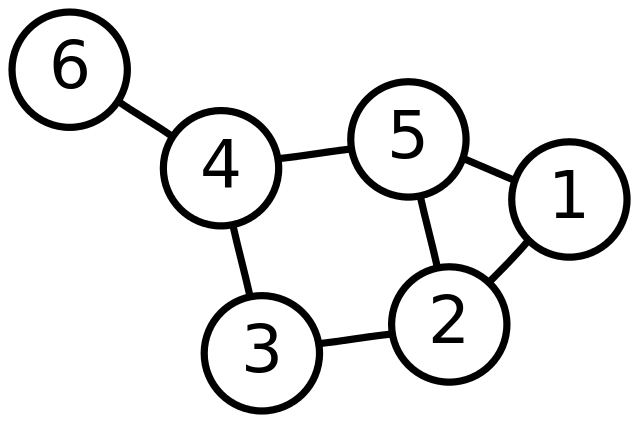
\includegraphics[width=0.4\textwidth]{graph-example}
        \caption{[TODO ]}
        \label{img:graph_example}
      \end{figure}

      \paragraph{}
      Aquellos grafos para los cuales la arista $e_j$ representa los dos sentidos de la relación, es decir, $v_{i_1}$ está relacionado con $v_{i_2}$ y $v_{i_2}$ está relacionado con $v_{i_1}$ se denominan \emph{Grafos no nirigidos}, mientras que en los casos en que esta relación no es recíproca se habla de \emph{Grafos dirigidos}. Cuando cada arista $e_j$ tiene asociado un determinado peso $w_j \in W =  \{ w_1, w_2, ..., w_m\}$ se dice entonces que $G$ es un \emph{grafo ponderado} mientras que cuando se presupone que todas las aristas tienen el mismo peso se omite dicha notación.

      \paragraph{}
      Cuando un vértice denominado $v_{i_1} \in V$ está directamente relacionado con otro denominado $v_{i_2} \in V$, es decir, existe una arista $e_j \in E$ que los conecta ($e_j = (v_{i_1}, v_{i_2})$) se dice que son $e_j$ es \emph{incidente} de dichos vértices. De la misma manera se dice que $v_{i_1}$ y $v_{i_2}$ son \emph{adjacentes} entre sí.

      \paragraph{}
      Respecto del número de aristas incidentes sobre cada vértice, se denomina \emph{grado} al cardinal de estas, diferenciando en los grafos no dirigidos entre \emph{in-grado} a las de destino y \emph{out-grado} a las de salida. Se utiliza la notación $d(v_i)$ para referirse al grado del vértice i-ésimo, $d^+(v_i)$ al \emph{in-grado} y $d^-(v_i)$ al \emph{out-grado} de dicho vértice. Nótese que se cumple la siguiente propiedad: $d(v_i) = d^+(v_i) + d^-(v_i)$.


      \paragraph{}
      Un \emph{camino} es un conjunto de aristas $P_p = \{ e_{k_1}, e_{k_2}, ..., e_{k_p}\}$ tales que la arista k-ésima tiene como vércice de destino el mísmo que utiliza la $k+1$ como vércice origen. Nótese que el valor $p$ indica la \emph{longitud} del camino. Cuando el vértice de destino de la arista $e_{k_p}$ es el mismo que el de origen de $e_{k_1}$ se denomina \emph{ciclo} y se denomina $C_p$.

      \paragraph{}
      Se denomina $K_n$ al grafo compuesto por $n$ vértices y $n*(n-1)$ arístas de tal manera que estas conectan cada vértice con todos los demás. Nótese que este número se reduce a la mitad en el caso de los grafos no dirigidos.

      \paragraph{}
      Cuando en un grafo al estudiar la estructura de un grafo, se comprueba que el conjunto de vértices puede dividirse en dos subconjuntos disjuntos $V_1$ y $V_2$ de tal manera que para todas las aristas $e_j = (v_{i_1}, v_{i_2})$ el vértice $v_{i_1}$ se encuentra en el subconjunto $V_1$ y el vértice $v_{i_2}$ se encuentra en el subconjunto $V_2$, entonces se habla de un \emph{Grafo Bipartito}. Un ejemplo de esta situación se muestra en la figura \ref{img:bipartite_graph_example}.

      \begin{figure}
        \centering
        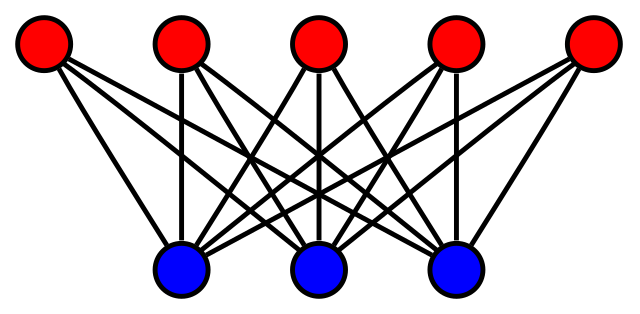
\includegraphics[width=0.4\textwidth]{bipartite-graph-example}
        \caption{[TODO ]}
        \label{img:bipartite_graph_example}
      \end{figure}

      \paragraph{}
      Un \emph{subgrafo} $H$ es el grafo compuesto por un subconjunto de vectores y aristas del grafo $G$. Nótese que en el caso de que eliminen vértices, es necesario eliminar también todas sus aristas incidentes. Esto se puede indicar de manera matemática de la siguiente forma: $H \subseteq G$ por lo que $H_V \subseteq G_V$ y $H_E \subseteq G_E$.

      \paragraph{}
      [TODO hablar sobre transformaciones en grafos]

      \subsection{Métodos de Representación}
      \label{sec:laplacian_matrix}

        \paragraph{}
        [TODO ]

        \subsubsection{Matriz de Adyacencia}
        \label{sec:adjacency_matrix}

          \paragraph{}
          [TODO ]

        \subsubsection{Lista de Adyacencia}
        \label{sec:adjacency_list}

          \paragraph{}
          [TODO ]

      \subsection{Matriz Laplaciana}
      \label{sec:laplacian_matrix}

        \paragraph{}
        [TODO ]

    \section{Problemas sobre Grafos}
    \label{sec:graph_problems}

      \paragraph{}
      [TODO ]

      \subsection{Matching}
      \label{sec:graph_matchings}

        \paragraph{}
        [TODO ]

      \subsection{Arbol Recubridor Mínimo}
      \label{sec:minimum_spanning_tree}

        \paragraph{}
        [TODO ]

      \subsection{Problemas de Rutado}
      \label{sec:network_routing}

        \paragraph{}
        [TODO ]

      \subsection{Problemas de Cubrimiento}
      \label{sec:network_covering}

        \paragraph{}
        [TODO ]

      \subsection{Análisis de Redes}
      \label{sec:network_analysis}

        \paragraph{}
        [TODO ]

    \section{Modelo en Semi-Streaming}
    \label{sec:semi_streaming_model}

      \paragraph{}
      [TODO]

    \section{Sparsification}
    \label{sec:graph_sparsification}

      \paragraph{}
      [TODO]


    \section{Conclusiones}
    \label{sec:graphs_conclusions}

      \paragraph{}
      [TODO ]

\end{document}
